\subsection{Seeing transformations on one coordinate plane}

The formulas for graph transformations should be connected with a visible motion of the graph. The diagram below starts from
\[
f(x)=x^2
\]
and compares it with a vertical shift and a horizontal shift.

\begin{center}
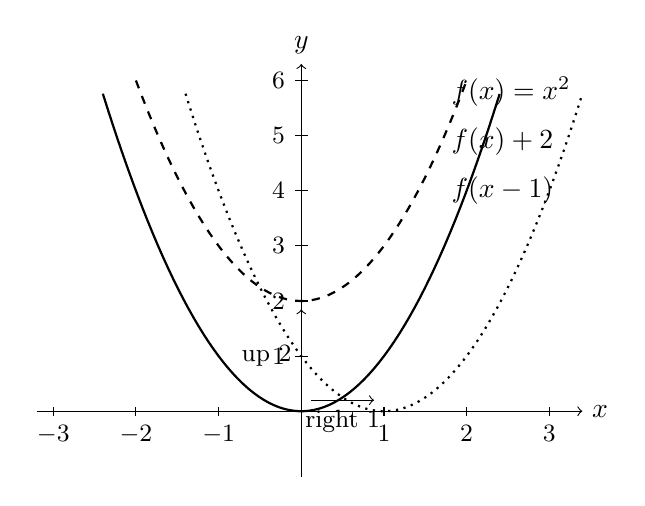
\begin{tikzpicture}[x=1.05cm,y=0.7cm]
  \draw[->] (-3.2,0) -- (3.4,0) node[right] {$x$};
  \draw[->] (0,-1.2) -- (0,6.3) node[above] {$y$};
  \foreach \x in {-3,-2,-1,1,2,3}
    \draw (\x,0.08) -- (\x,-0.08) node[below] {\small $\x$};
  \foreach \y in {1,2,3,4,5,6}
    \draw (0.08,\y) -- (-0.08,\y) node[left] {\small $\y$};

  \draw[thick,domain=-2.4:2.4,samples=80] plot (\x,{\x*\x});
  \draw[thick,dashed,domain=-2:2,samples=80] plot (\x,{\x*\x+2});
  \draw[thick,dotted,domain=-1.4:3.4,samples=80] plot (\x,{(\x-1)*(\x-1)});

  \node[anchor=west] at (1.7,5.8) {$f(x)=x^2$};
  \node[anchor=west] at (1.7,4.9) {$f(x)+2$};
  \node[anchor=west] at (1.7,4.0) {$f(x-1)$};
  \draw[->] (0,0.15) -- (0,1.85) node[midway,left] {\small up $2$};
  \draw[->] (0.12,0.2) -- (0.88,0.2) node[midway,below] {\small right $1$};
\end{tikzpicture}
\end{center}

\begin{interpretationbox}[Read the motion before memorising the formula]
Adding outside the function changes output values and therefore moves the graph vertically. Changing the input inside the function moves the graph horizontally, with the direction reversed in the notation: $f(x-1)$ moves the graph one unit to the right.
\end{interpretationbox}
